% Template for a Computer Science Tripos Part II project dissertation
\documentclass[12pt,a4paper,twoside,openright]{report}
\usepackage[pdfborder={0 0 0}]{hyperref}    % turns references into hyperlinks
\usepackage[margin=25mm]{geometry}  % adjusts page layout
\usepackage{graphicx}  % allows inclusion of PDF, PNG and JPG images
\usepackage{verbatim}
\usepackage{docmute}   % only needed to allow inclusion of proposal.tex
\usepackage{listings}

\raggedbottom                           % try to avoid widows and orphans
\sloppy
\clubpenalty1000%
\widowpenalty1000%

\renewcommand{\baselinestretch}{1.1}    % adjust line spacing to make
                                        % more readable

\begin{document}

\bibliographystyle{plain}

\lstset{basicstyle=\ttfamily, tabsize=2, columns=flexible, showstringspaces=false}
\newcommand{\code}{\lstinline}
\newcommand{\name}{\textsl}
\lstnewenvironment{xml}{\lstset{language=Xml, basicstyle=\ttfamily}}{}
\lstnewenvironment{ocaml}{\lstset{language=[Objective]Caml}}{}


%%%%%%%%%%%%%%%%%%%%%%%%%%%%%%%%%%%%%%%%%%%%%%%%%%%%%%%%%%%%%%%%%%%%%%%%
% Title


\pagestyle{empty}

\rightline{\LARGE \textbf{Joel Jakubovic}}

\vspace*{60mm}
\begin{center}
\Huge
\textbf{An XMPP Server Implementation In OCaml} \\[5mm]
Computer Science Tripos -- Part II \\[5mm]
Pembroke College \\[5mm]
\today  % today's date
\end{center}

%%%%%%%%%%%%%%%%%%%%%%%%%%%%%%%%%%%%%%%%%%%%%%%%%%%%%%%%%%%%%%%%%%%%%%%%%%%%%%
% Proforma, table of contents and list of figures

\pagestyle{plain}

\chapter*{Proforma}

{\large
\begin{tabular}{ll}
Name:               & \bf Joel Jakubovic                         \\
College:            & \bf Pembroke  College                      \\
Project Title:      & \bf An XMPP Server Implementation In OCaml \\
Examination:        & \bf Computer Science Tripos -- Part II, July 2017  \\
Word Count:         & \bf About 7000\footnotemark[1]
                      (well less than the 12000 limit)  \\
Project Originator: & Dr Anil Madhavapeddy \& Dr Richard Mortier           \\
Supervisor:         & Richard Mortier                    \\
\end{tabular}
}
\footnotetext[1]{This word count was not yet computed
by \texttt{detex diss.tex | tr -cd '0-9A-Za-z $\tt\backslash$n' | wc -w}
}
\stepcounter{footnote}


\section*{Original Aims of the Project}

To use the OCaml language and its libraries to build a server implementing the XMPP protocol \ldots conforming to the core XMPP spec as well as the XMPP-IM extension spec.

\section*{Work Completed}

A server, implementing basic XMPP functionality, including message forwarding to clients and presence notification according to subscription between clients. A simple client was also developed for testing purposes, and its bytecode form is interactively usable in the OCaml toplevel.

\section*{Special Difficulties}

None? (I feel like there was a primary special difficulty, namely that XMPP is a huge and complicated protocol and that the RFCs are tedious to get through.)

Interesting: \textit{``It is quite in order for the Proforma page to point out \textbf{how ambitious} the original aims were, and how the work completed represents the triumphant consequence of \textbf{considerable effort against a background of unpredictable disasters}. The substantiation of these claims will follow in the rest of the dissertation.''} -- Pink Book

\newpage
\section*{Declaration}

I, Joel Jakubovic of Pembroke College, being a candidate for Part II of the Computer
Science Tripos, hereby declare
that this dissertation and the work described in it are my own work,
unaided except as may be specified below, and that the dissertation
does not contain material that has already been used to any substantial
extent for a comparable purpose.

\bigskip
\leftline{Signed Joel Jakubovic}

\medskip
\leftline{Date [date]}

\tableofcontents

%%%%%%%%%%%%%%%%%%%%%%%%%%%%%%%%%%%%%%%%%%%%%%%%%%%%%%%%%%%%%%%%%%%%%%%
% now for the chapters

\pagestyle{headings}

\chapter{Introduction}
The eXtensible Messaging and Presence Protocol (XMPP) is designed for securely passing XML messages between clients and servers. Amongst its services are ordinary instant-messaging functionality, storage of contacts, discovery of online status of users, and push-based notifications. Google and Apple employ it for the latter use, and it is central to the well-known WhatsApp messaging application. \ldots

\chapter{Preparation}
For the bulk of the preparatory work, the clue was in the title: I needed to be familiar with OCaml and XMPP. This involved maintaining a basic level of competence with OCaml language features, as well as experience with the libraries and tools I was going to use; understanding of the basic concepts of XML, and which features are relevant to XMPP; then, the details of the XMPP protocol itself. Once I had a vision of what would be needed, I could design the general architecture of the server.

\section{Starting point}
I relied on the existing OCaml platform, including its standard libraries and others such as Angstrom.

\section{The OCaml language}
Objective-Caml, or OCaml, is a primarily functional language with imperative and object-oriented features. I had already used OCaml, to a basic extent, on an internship during the summer; this had given me some experience with the Angstrom parser combinator library. I referred to Internet resources and the \name{Real World OCaml} book to re-familiarise myself and fill the gaps in my knowledge.

I surveyed the documentation for the \code{Unix} module, to remind myself of how the Sockets API operates. I then put together a couple of small test servers and clients to verify I could use the networking functions from OCaml correctly. This also provided an opportunity to get used to the build system again.

I also browsed the small standard library for data structure implementations. All of the basic ones exist, and more specialised versions are provided in external libraries should I need them.

The server needed to handle many clients at once, so I needed some form of multitasking. OCaml offers two co-operative threading libraries, \code{Lwt} and \code{Async}, in addition to an interface to POSIX pre-emptive threads. When I later had to adapt my single-threaded code to serve multiple clients, I chose POSIX threads, since the pre-emptive multithreading approach was already familiar to me and I did not need to make serious modifications to the code I had already written.

\section{XML}
XML is a notation for hierarchical trees, and an XML node \footnote{Technically, there are also text nodes: as XML was designed as a markup language, any point in the tree can be made up of text, or `content'.} has the form
\begin{xml}
<prefix:tag pre1:attr1="value1" pre2:attr2="value2" ... pren:attrn="valuen" >
   ... children ...
</prefix:tag>
\end{xml}
where \code{attr}\(i\) are the node's attributes. Most of the time, prefixes are absent from attributes, but they are used in a couple of important cases outlined below. I call the combination of prefix and identifier a \emph{qualified name}. This way, a node can be seen as
\begin{xml}
<qname qname1="value1" qname2="value2" ... qnamen="valuen" >
  ...
</qname>
\end{xml}

\subsection{Namespaces}\label{sec:namespaces}
Namespaces are a way to organise tags and avoid naming conflicts in XML; each tag is qualified by a namespace. Namespaces are typically long strings, and it would be cumbersome to work with XML where every single tag had such a namespace concatenated onto it. Instead, a shorthand for the namespace is prefixed onto tags. The association between a prefix and the namespace it represents is defined by an (ab)use of the XML attribute system: the `attribute' \code{xmlns:foo="bar"} is treated specially as saying that the prefix \code{foo} represents the namespace \code{bar}. A tag can in fact forego a prefix, in which case it is considered to use the default prefix, signified by \code{xmlns="bar"}. These associations are local to the node in the tree and are inherited by its children.

There are other special `attributes' in this fashion, such as \code{xml:lang}, which specifies the language used for plain text within the subtree it is part of. I deemed the possibly many other special attributes not relevant to this project. Nor did I concern myself with other beauraucratic details such as file encoding, validation via XML schemas or comments / \code{CDATA} sections.

\subsection{Formal grammar for XML}
I developed the following informal Context-Free Grammar for this subset of XML, to guide my implementation of the parser:

\begin{minipage}{\linewidth}
  \begin{lstlisting}
  qname    ::= (ident ':')? ident
  attr_val ::= qname '=' '"' string '"'
  branch   ::= '<' qname attr_val* tag_end
  tag_end  ::= '/>'
             | '>' node '</' qname '>'

  node  ::= branch
         | text

  \end{lstlisting}
\end{minipage}

In the CFG, \code{ident} denotes an identifier, \code{string} represents a text string containing appropriately escaped quote characters, and \code{text} refers to free text not containing angle bracket characters. This was strictly a guide, to give the general shape of the syntax. Obviously XML parsing is not \emph{truly} context-free as the closing tag must match the opening tag; nevertheless, such a grammar is still useful.

\section{The XMPP Protocol}

\subsection{Understanding the protocol}
The most comprehensive and in-depth resource on XMPP is the specification, RFC 6120. My first attempt at understanding XMPP involved trying to read this document. Since at first all I wanted was a broad picture, I found the book \name{XMPP: The Definitive Guide} to be a more appropriate resource.

Once I had a broad overarching understanding, the only place I could start with was the communications setup and handshake. The \name{Definitive Guide} was helpful, but for the details I had to delve into the RFC. I quickly realised that XMPP is a very large and complex protocol, and I would have to prioritise the aspects that would get me to a message-processing stage as fast as possible. In other words, I needed to adopt a breadth-first, and not depth-first, approach to both understanding XMPP and implementing a server for it. Thus, for each feature of the protocol, I pressed ahead with the core behaviour first. The specification contains a rather overwhelming range of error cases and caveats for most aspects of XMPP, and I would treat these details as extension work for any remaining time at the end.

To help guide me through the relevant sections of RFC 6120, I downloaded the XMPP client program Psi\cite{Psi-IM} and learned its basic use. I would treat Psi as a typical client and make the server conform to the data it sent.

What follows in subsequent sections is my consideration of specific parts of XMPP, and the design decisions affecting their representation in my server.

\subsection{Handshake and setup considerations}
Outline:
\begin{itemize}
  \item Exposition of Section \ref{sec:server-setup}; the basic steps in setting up an XMPP session
  \item Not bothering with authentication, encryption ... all extraneous and viewed as extensions.
  \item Stream errors and disconnection
\end{itemize}

\subsection{The roster}
`Roster' is simply XMPP jargon for what is functionally a contact list. XMPP represents a user's contacts as a list of \code{<item>} elements. Each item describes another user, and the subscription status between the two users.

The concept of subscription has design ramifications worth discussing. The word is used in its usual sense: if user A is subscribed to user B, then A will receive updates about B's presence on the network. This is a \emph{directed} relation; B might not be subscribed to A. Thus, conceptually, subscription is a directed graph that needs to be stored on disk as well as in memory. There is, then, a choice of how to represent this graph.

The two main options for graph representation are \emph{adjacency list} and \emph{adjacency matrix}.

An adjacency matrix, being a conceptually two-dimensional structure, would have forced me to think about implementation in terms of nested one-dimensional maps or arrays. This would complicate the issue of avoiding loading the entire graph at once, and hence how to split it into separate files or regions of a file, and so on. On the other hand, an adjacency list for each node would be simple to implement using conventional files and in-memory data structures. Furthermore, this already matches up to the way XMPP treats the subscription relation; a list of contacts per user. When the user connects, simply load the list.

Thus, I picked the adjacency list. I would have a separate file for each `vertex' of the graph, in a format resembling a list of \code{<item>}s, and similar separate in-memory data structures, making loading and lookup simple to think about.

For example, the username \code{alice} has a roster file located in the \code{roster/} directory called \code{alice.xml}. It consists of a list of XMPP roster \code{<item>} elements.

The subscribers of user A are recorded in the XMPP \code{<item>} elements as \code{from}, \code{to}, or \code{both}. RFC 6121 defines \code{to} as A having a subscription to the user in the \code{<item>} element; \code{from} is the converse, and \code{both} simply means A and B are mutually subscribed.

Now, if A's roster (on disk or in memory) says it is subscribed \code{to} B, then B's roster should say it is subscribed \code{from} A. The analogous case applies to \code{from}/\code{to}. This is an invariant that must be maintained if the roster, taken as a whole, is to be consistent, and is a consequence of the adjacency list representation.

[but --- no need to enforce, since I abandoned CRUD operations and can trust my own files to be consistent]
However, I viewed supporting CRUD (Create, Read, Update, Delete) operations for the roster as extension work, since implementing them before messaging would be too time consuming. The rosters are determined by the content of the roster files which I ensure are consistent myself, and since they do not change during runtime or get updated by the server, this consistency is maintained.

\subsection{Messaging and stanzas}
Outline:
\begin{itemize}
  \item Sticking to simple messages with \code{to}, \code{from}, \code{type} attributes; oblivious to nested XML, simply pass along
  \item Sticking to online-offline (\code{avaliable} / \code{unavailable}) presence notification only
  \item Sticking to single-server model; i.e. no federation (``yet'')
  \item Only implementing the \code{iq} stanzas necessary for handshake; too many potential services otherwise. Graceful (spec-sanctioned) error response (\code{feature-unavailable} error stanza) so that more feature-rich clients (read: Psi) can still continue to operate with the server.
\end{itemize}

\subsection{Multi-client architecture}
This section is supposed to explain the design behind Section \ref{sec:mod-dispatch} (dispatch machinery) as well as
\begin{itemize}
  \item Developed first for a single client; multiple clients perform the same actions specified by the same function, just in  different thread
  \item Design of the testing clients; explaining the analogous Section \ref{sec:mod-client} in Implementation, as well as the test rig
\end{itemize}


\chapter{Implementation}
As the objective of this project was to build a server, I developed a server program (\code{server.ml}). I used the Psi client software to help develop the server, but for later testing a more automatable client was needed. For this reason, I also developed a basic XMPP client controller (\code{client.ml}).
These both make heavy use of the \code{Xml} and \code{Xmpp} modules.

\section{The \code{Xml} module}\label{sec:xmlmod}
XML is central to XMPP. In my code, it comes in three main forms: as text, as low-level `Raw' XML, and as high-level \code{xml_node}. The \code{Xml} module provides utilities for working with these representations.

Both explicit and default prefixes\ref{sec:namespaces} are used throughout XMPP. When starting out, I assumed that the particular prefix used on some element would not matter. For instance, the \code{<body>} element of HTML could be written \code{<html:body>} (as long as the \code{html} prefix referred to the HTML namespace), \code{<body>} (provided HTML was the default namespace), or even \code{<quux:body>} (if \code{quux} referred to the HTML namespace). However, XMPP provides at least one exception to this: the initial \code{<stream>} element needs to use the \code{stream:} prefix. So, a distinction between namespaces and their prefixes was preserved at some level of the system. However, in the other 99\% of cases, I considered it sufficient to place constraints only on the namespace and tag, hence why the XML checking functions are prefix-agnostic.

XML-as-text is suitable only for human comprehension; computationally, being a long unstructured block of bytes, it is unsuitable for computer processing. XMPP, though, is built around sending and receiving XML via text, so the ability to parse incoming XML and output XML text was fundamental. The \code{Xml.P} module contains Angstrom parsers for XML syntax, producing a `literal' abstract representation defined in \code{Xml.P.Raw}. Functions for converting this back into text, for output purposes, also live in \code{Xml.P.Raw}.

The main Angstrom parser is \code{tree}, which converts nested opening/closing tags and embedded text into a \code{Raw.Branch} node, or \code{Raw.Text} if the whole thing consists of just text. This suffices for most of XMPP, but there are some situations that do not involve fully completed trees. For example, setting up the client-server XML stream involves only the opening tag of the \code{<stream>} element; likewise, terminating the stream requires the closing tag. Thus, I included \code{tag_open} and \code{tag_close}. In addition, before opening the stream, an XML declaration \code{<?xml version="1.0"?>} is needed, which uses slightly different syntax to XML tags. Since this syntax does not appear anywhere else, I used a custom parser for this purpose.

These parsers are all implemented in terms of smaller named parsers, combined using the Angstrom parser combinators. For example, I defined \code{tag_open} this way:

\begin{ocaml}
let tag_open =
  tok_langle *> qual_name >>= fun (ns,id) ->
    lift2 (fun attrs _ -> Raw.Branch ((ns,id,attrs),[]))
      (many attr_val)
      tok_rangle
\end{ocaml}

This can be read as: ``Accept the token \code{<}, then a qualified name, then zero or more attribute-value pairs, then the token \code{>}; combine the qualified name and the attributes into a \code{Branch} node with no children''. To elaborate: \code{tok_langle = lex (char '<')}, \code{tok_colon = lex (char ':')}, and so on, where \code{lex} skips whitespace.

The parsers written in this manner resemble the Context-Free-Grammars of XML structures, although the choice operator \code{<|>} is an ordered choice. This shows itself in my implementation of \code{tree}:

\begin{ocaml}
let tree = fix ( fun t_rec ->
  ( tok_langle *> qual_name >>= fun (ns,id) ->
          lift2 (fun attrs children -> Raw.Branch ((ns, id, attrs), children))
            (many attr_val)
            (tok_leaf *> return [] <|> tok_rangle *> branch t_rec (ns,id)) )
  <|> (take_while1 (function | '<' -> false | _ -> true) >>| Raw.text) )
\end{ocaml}

As an XML node can be simple text, this is accounted for by assuming text content when an attempt to parse a tag fails.

[should I include more on parsers?]

\subsection{The \code{Raw} module}
As mentioned, the \code{Raw} module contains the `literal' abstract XML representation that these parsers target. Consider

\begin{xml}[label={lst:xmlsample}]
<foo:error type="fatal" xmlns:foo="long-application-namespace" >
  <a></a>
  <b></b>
  Sample text
</foo:error>
\end{xml}

The parent node has a qualified tag \code{foo:error}, along with a list of attributes. Each attribute conceptually consists of a prefix, name and value. The prefix might be empty, such as the case of \code{type="fatal"}. The first task of abstract representation is to make all of these explicit, representing attributes as pairs of qualified names and values. \code{type="fatal"} and \code{xmlns:foo="bar"} become the list
\begin{lstlisting}
[ (("", "type"), "fatal"); (("xmlns", "foo"), "bar") ]
\end{lstlisting}
The above XML source would parse into the following \code{Raw.xml}:

\begin{ocaml}
Branch ( ("foo", "error", [
    (("", "type"), "fatal");
    (("xmlns", "foo"), "long-application-namespace")
  ]) , [
    Branch ( ("", "a", []) , []) ;
    Branch ( ("", "b", []) , []) ;
    Text "Sample text" ;
] )
\end{ocaml}

Note the `literal' interpretation of the attribute list as an actual OCaml list. Technically, the order of XML attributes does not matter, but it is simpler to use a list at this level. Also, the special considerations of namespaces and prefixes are not handled at this level; it sees \code{xmlns:foo="bar"} as just another attribute.

The \code{Raw} module provides functions to convert its data structures into strings. The main \code{to_string} function, which recursively serialises an XML tree, is as follows:

\begin{ocaml}
let rec to_string = function
  | Text str -> str
  | (Branch ((ns,tag,attrs),children)) as xml ->
    match children with
    | [] -> to_string_single (ns,tag,attrs)
    | _  -> let interior = String.concat "" (List.map to_string children) in
            to_string_open xml ^ interior ^ to_string_close xml
\end{ocaml}

An XML node without children can be written as \code{<node></node>}. However, it is legal to write such an empty node as \code{<node />}, which is often visually cleaner. This is what \code{to_string_single} does. Otherwise, the children are recursively serialised and enveloped in the opening and closing tags. [indentation?] [sanitisation?][more on \code{to_string_open}, \code{string_of_qname}, \code{string_of_attrs}]

\subsubsection{Utility constructors}
Initially, having the \code{Raw} representation and its serialisation functions, I simply used them to generate the server responses. However, many elements needed at least a default namespace, all prefixes needed to be explicitly specified, and the syntax was very heavy to write and read:

\begin{ocaml}
respond_tree
  (X.Xml (("stream","features",[]),[
    X.Xml (("","mechanisms",[(("","xmlns"),Xmpp.sasl)]),[
        X.Xml (("","mechanism",[]),[ X.Text "PLAIN" ]);
        X.Xml (("","required",[]),[])
      ])
  ]));
\end{ocaml}

After consideration, I reasoned that it would be easier in the long run to add some conveniences for such construction of XML trees in OCaml code. Firstly, I wanted to avoid writing prefixes. The tags mostly use the default (empty) prefix, and the only attribute prefix that is ever used is \code{xmlns:}. By handling namespaces in a more convenient fashion, I could avoid having to specify prefixes for both tags and attributes altogether.

For the purposes of output, I committed to using only one, standard prefix per namespace (recall that prefixes are local to parts of a tree, but such freedom is not really needed here). I bundled namespaces and prefixes together, so that I could refer to them by a simple OCaml identifier. For example, the opening \code{<stream:stream>} element uses the stream prefix, referring to the namespace \code{http://etherx.jabber.org/streams}. I made definitions (in the \code{Xmpp} module) like so:

\begin{ocaml}
let jstream  = ("stream","http://etherx.jabber.org/streams")
let jclient  = ("client","jabber:client")
let jserver  = ("server","jabber:server")
\end{ocaml}

Other namespaces were only ever used with the default (empty) prefix. I did the same with them:

\begin{ocaml}
let streams = ("","urn:ietf:params:xml:ns:xmpp-streams")
let session = ("","urn:ietf:params:xml:ns:xmpp-session")
let sasl    = ("","urn:ietf:params:xml:ns:xmpp-sasl")
let bind    = ("","urn:ietf:params:xml:ns:xmpp-bind")
...
\end{ocaml}

I developed convenience functions to construct XML trees using this: \code{xml_d}, \code{xml}, \code{xml_n}, and \code{text}.

For \code{xml_n}, the \code{n} stands for ``no namespace''. This is used for child XML that does not use namespaces at all. For example, the following:
\begin{ocaml}
xml_n "rectangle" [ "width", "240"; "height", "180" ] [
  text "Sample text"
]
\end{ocaml} constructs the \code{Raw.xml}
\begin{ocaml}
Raw.Xml (("","rectangle",[(("","width"),"240"); (("","height"),"180")]),[
  Raw.Text "Sample text"
]
\end{ocaml}

\code{xml_d} means `declare'. It is similar to \code{xml_n}, but accepts a prefix-namespace pair. It applies the prefix to the tag and declares the association between prefix and tag in the attributes, automatically. This means that example \ref{lst:xmlsample} could be constructed like so:

\begin{ocaml}
module Xmpp = struct
  ...
  let foo = ("foo", "long-application-namespace")
  ...
end

xml_d Xmpp.foo [ "type", "fatal" ] [
  xml_n "a" [] [];
  xml_n "b" [] [];
  text "Sample text"
]
\end{ocaml}

Finally, \code{xml} is a somewhat idiosyncratic variant that exists for child XML that can use a prefix, but does not declare it. [made sense at the time ... rather obscure motivation. probably worth leaving out --- though it \emph{is} used in code samples!]

The advantages of this notation are clear: high signal-to-noise ratio\footnote{OCaml's data constructors are not curried, requiring parentheses, whereas function application does not require them. Also, in some situations, such as lists, it is legal to drop parentheses in pairs: \code{[ (x,y); (z,w) ]} becomes \code{[ x,y; z,w ]}.}, and the use of functions allows automatic handling of namespaces. The end result is that the code finally looks somewhat like the thing it represents.

\subsection{High-level \code{xml_node}}
The higher-level representation, \code{xml_node}, exists for situations where \code{Raw}'s data structures become unwieldy. It is defined as follows:

\begin{ocaml}
type xml_node =
| Text of lang * string
| Xml of {
  tag    : qname;
  attr   : string -> string option;
  attr_full : qname -> string option;
  namespace : string -> string option;
  lang  : lang;
  child : xml_node list;
  orig  : P.Raw.xml;
}
\end{ocaml}

The main improvement is the use of an opaque attribute lookup function, rather than an explicit data structure. \code{attr_full} takes a qualified name, but since most attributes do not have a namespace prefix, the more convenient attr is also provided. \code{attr} is implemented as calling \code{attr_full} with an empty namespace prefix.

One consideration with namespaces is that prefix-namespace mappings are inherited to child nodes of their declaration site. \code{xml_node} incorporates this functionality into the namespace function. It finds the namespace associated with a prefix, delegating to the parent node if unsuccessful. [expand on how exactly I accomplished this]

\code{attr}, \code{attr_full} and namespace all internally use the standard library's \code{Map} structure, being more appropriate for lookup than lists; lists require a linear scan to locate a mapping, and a full scan of the list to determine its absence, whereas \code{Map} provides logarithmic-time lookup.

An \code{xml_node} is constructed from an original \code{Raw.xml} structure, and it is useful to keep this information for output purposes. It is stored in the \code{orig} field.

The language of any text content is, like namespaces, an inherited special attribute, and is signified by \code{xml:lang} in the attribute list. It is stored in the \code{lang} field of the branch, and propagated to leaf \code{Text} nodes. This is because a \code{Text} instance, in isolation, does not have a reference to its parent, and hence must have its own \code{lang} attribute.

The construction of an \code{xml_node} from \code{Raw.xml} is accomplished by the \code{from_raw_br} function. [how much detail to go into on this?]

\subsubsection{Semantic checking and matching} \label{sec:matchers}
The text-to-\code{Raw} parsers solve the problem of structuring XML and detecting syntax errors; after all, not all text is valid XML. However, XMPP is a protocol over XML and hence imposes a second level of `syntax' on top of this. So, in a similar way, not all valid XML is valid XMPP. But this does not entail further structuring of the XML; rather, it mainly involves checking that certain tags or attributes are present, and extracting values of attributes or embedded text nodes --- this problem is one of ``pattern matching'' rather than parsing. OCaml's built-in pattern matching proved not to be suitable for this purpose [and would not work with the high-level rep anyway; perhaps I should prioritise this reason], so I went down the route of parsers and combinators modelled after Angstrom.

Unlike Angstrom's parsers, which are designed to be fairly orthogonal fundamental building blocks of more complex parsers, mine are deliberately special-purpose. I went with whatever would be useful to write readable code, without necessarily being exhaustive in the range of behaviours achievable by combining them.

I viewed a `matcher' as a function accepting an \code{xml_node} and returning a \code{Result} value. Composition of matchers was then to involve both composition of functions, and composition of \code{Result} values\footnote{The resulting library could be seen as a fusion of the Function and \code{Result} monads.}. Application of a matcher to an \code{xml_node} is simple function application.

The matchers live in the \code{Xml.Check} module. The main ones are \code{tag} / \code{qtag}, \code{attr} / \code{attr_opt}, \code{attv}, \code{child} / \code{children}, \code{orig} and \code{text}.

\begin{itemize}
  \item \code{tag "message"} succeeds if the node has the \code{message} tag

  \item \code{qtag} functions like \code{tag}, but takes a namespace prefix to also check

  \item \code{attr "id"} results in the value of the \code{id} attribute if it exists

  \item \code{attv "id" "1234"} succeeds if the \code{id} attribute exists and is equal to 1234

  \item \code{attr_opt} is like \code{attr} but does not fail, instead resulting in \code{Some <value>} or \code{None}

  \item \code{child} gives the first child of the node if it exists

  \item \code{children} gives a list of the node's children (possibly the empty list, so this one also never fails)

  \item \code{orig} results in the low-level \code{Raw} representation from which the \code{xml_node} was obtained

  \item \code{text} gives the text string of a \code{Text} node
\end{itemize}

I avoid using the word `return' here, as strictly what these functions return is a \code{Result}, possibly containing the `resulting' value --- or an error. For those that merely check some condition rather than retrieve a value (\code{tag}/\code{qtag} and \code{attv}), I say they `succeed' instead\footnote{This could mean `resulting' in the value \code{()}, but I actually found it more useful to `result' in the \code{xml_node} passed in.}.

\subsubsection{Matcher combinators}
The combinators let me write XML matching code resembling, as closely as possible in OCaml\footnote{Short of syntax extensions perhaps, which I am unfamiliar with}, the XML itself:

\begin{ocaml}
tag "iq" *> attv "type" "get" *> attr "id" >>= fun id ->
  (* id is now bound to the "id" attribute *)
  ...
\end{ocaml}

This would succeed on the XML node
\begin{lstlisting}[language=xml]
<foo:iq type="get" id="123" > ... </foo:iq>.
\end{lstlisting}

I implemented the usual \code{>>=} for `bind', \code{*>} for `sequence', \code{<|>} for `alternative' and the direction-reversed versions where needed.

\begin{itemize}
  \item \code{(f >>= fun x -> g) xml} first performs \code{f xml}; if successful, it binds the result value to \code{x} and returns \code{g xml}. Otherwise, if \code{f xml} fails, it aborts with the error value.

  \item \code{(f *> g) xml} is like \code{>>=} but discards the result, binding no values. In this sense, it sequences a `check' with a check or match, although this is a conceptual distinction that is not enforced in the code.

  \item \code{(f <|> g) xml} is like \code{*>}, but with opposite error behaviour: when \code{f xml} fails, \code{g xml} is tried.
\end{itemize}

The matcher implementations are all fairly straightforward and similar to each other. For instance, \code{attr}:

\begin{ocaml}
let attr k = function
  | Xml xml -> (match xml.attr k with
    | Some v -> Ok v
    | None -> Error (format "Expected %s attribute in <%s> tag" k (snd xml.tag)) )
  | Text _ -> Error "Expected XML, not content"
\end{ocaml}

Out of the above matchers, only \code{text} makes sense for text nodes. Because both the low- and high-level XML types incorporate the possibility of text, all matchers except \code{text} have to account for this case at runtime.

\subsubsection{The question of buffering}
Angstrom provides the \code{parse_only} function for parsing an in-memory string in its entirety. But in this application, such a mode is not possible. First, from a remote source on the network, completed XML might arrive in several bursts of data rather than all at once. Second, most XML takes the form of stanzas, which need to be parsed and processed one-by-one as they come. This all points to some sort of `incremental' parsing functionality, requiring buffering of XML from outside. Fortunately, Angstrom's \code{parse} function produces a state that can be progressively fed input until it finishes.

From the beginning, I found it useful to employ an ``expect-input, respond-output'' model for the conversational bulk of the server and client code (such as the initial handshake). Functions for responding to the client were simple, generally consisting of output to a channel plus a flush of the channel. The `expect' function, though, was more involved.

Angstrom's \code{Buffered} interface maintains an internal buffer, of type \code{Bigstring}. After a successful parse, some of the data in the buffer may be unconsumed. It is the caller's responsibility to ensure parsing continues where it left off, and this is handled by the function passing the relevant sub-buffer each time it is needed. When everything has been consumed, the buffer needs refilling from the network. Unfortunately, the standard library's \code{input} function reads data into a \code{Bytes}-type buffer and not a \code{Bigstring}. To bridge this gap, I split my originally desired 1024-byte buffer into a \code{Bytes} and \code{Bigstring} of 512 bytes each. \code{input} reads into the \code{Bytes}, which is then blitted to the \code{Bigstring}, which can then be passed to Angstrom for parsing.

The user-level \code{expect} function takes an Angstrom parser (usually \code{P.tree}) and tries to parse from these internal network-backed buffers. It returns a \code{Result} value, and is often used in tandem with the high-level XML functions like so:

\begin{ocaml}
expect P.tree >>| Xml.from_raw >>= fun high_level_xml_node -> ...
\end{ocaml}

\section{The \code{Xmpp} module}
This module is for common functionality more specific to XMPP than XML, although the line is arbitrary. The main functionality here is roster management, and recognition of stanzas. As mentioned in \ref{sec:xmlmod}, the prefix-namespace pairs used often in XMPP are defined here.

\subsection{The Roster}
There is conceptually a mapping from user to their roster. I found it useful to view a user's roster as another mapping, from a contact's JID to their \code{<item>} record. The user-roster association is a global \code{Map} data structure, and the roster itself is another \code{Map}.

I represented \code{<item>} records, in-memory, as follows:

\begin{minipage}{\linewidth}
  \begin{ocaml}
    type item = {
      jid     : string;        (* Contact's Jabber ID                       *)
      name    : string;        (* Human-friendly name of contact            *)
      recv_ok : bool;          (* OK to receive presence from this contact? *)
      send_ok : bool;          (* OK to send presence to this contact?      *)
      groups  : string list; (* Membership of contact in groups           *)
    }
  \end{ocaml}
\end{minipage}

This is almost a direct XML-to-OCaml translation of XMPP's \code{<item>} element, the main difference being my treatment of the \code{subscription} attribute. I felt that the \code{subscription} attribute as \code{none}, \code{from}, \code{to} or \code{both} was an odd and hard-to-remember way of representing subscription. The system thus translates this field into two boolean conditions: \code{recv_ok} (activated by \code{to} and \code{both}) and \code{send_ok} (activated by \code{from} and \code{both}). This was better for the uses to which the roster is put: when wishing to send presence notifications, I simply check whether it is OK to send, via \code{send_ok}, rather than mentally decrypting `to' or `from'. [as for groups, I had to abandon them because of time]

Rosters are managed through the \code{Roster} sub-module. After authenticating a client, the server calls \code{Roster.load_from_storage} with their username, to ensure that their contact information is available.

\code{Roster.load_from_storage} uses Angstrom parsers and the high-level \code{xml_node} interface to load the roster file into memory. The only part of this that is slightly interesting is \code{item_of_xml}, which constructs an item record from what should be an \code{<item>} XML node:

\begin{ocaml}
let item_of_xml =
  let open Xml.Check in
  tag "item" *> attr "jid" >>= fun jid ->
    attr "name" >>= fun name ->
      attr_opt "subscription" >>= ( function
      | None        -> pure (false,false)
      | Some "none" -> pure (false,false)
      | Some "to"   -> pure (true,false)
      | Some "from" -> pure (false,true)
      | Some "both" -> pure (true,true)
      | _ -> fail "Unknown subscription type" ) >>=
  fun (recv_ok,send_ok) ->
    pure { jid; name; recv_ok; send_ok; groups=[] }
\end{ocaml}

This demonstrates the utility of the \code{xml_node} matchers discussed in \ref{sec:matchers}. This function treats the absence of a \code{subscription} attribute as equivalent to \code{subscription="none"} (hence the use of \code{attr_opt}). \code{groups} is set to an empty value for the aforementioned reasons. There is also a corresponding \code{to_xml} function acting on \code{item} structures.

[abandonment of CRUD, view towards testing]

\subsection{The \code{Stanza} module}
Outline:

\begin{itemize}
  \item Meant to bring stanza formats into the type level

  \item \code{Iq} sub-module has \code{Iq.t} (record with request ID and further data dependent on the \code{type} attribute) and \code{Iq.of_xml}

  \item Did not extend with \code{Message} / \code{Presence} sub-modules since they are not as general or varied as \code{Iq}; managed fine without type-level message or presence stanzas
\end{itemize}

\section{The server program}
\subsection{Work-dispatching machinery (the \code{Dispatch} module)}\label{sec:mod-dispatch}
On the server, per client, post-handshake; outline:

\begin{itemize}
  \item Sets up worker thread to forward stanzas to the client. Obtains stanzas via \code{dequeue_work} on work queue created by \code{client_connected}.

  \item Main thread reacts to messages arriving, forwards to appropriate worker thread by means of \code{dispatch <jid> <stanza>}

  \item Global \code{jid -> work-queue} map, protected by mutex

  \item Each work-queue has a \code{Queue} data structure and a \code{Condition} (`monitor' pattern) for `work available' plus its associated mutex. Also a `finished' boolean so worker thread can finish and quit gracefully.

  \item \code{dispatch} pushes the work to the appropriate queue, signalling `available'

  \item \code{dequeue_work} blocks waiting on `available'; if the `finished' flag is set, produces \code{None} after queue empties, signalling to the worker thread to exit. Otherwise, produces \code{Some <work>}

  \item \code{client_disconnected} sets the `finished' flag and signals, then removes client from the global map.
\end{itemize}

\subsection{Server operation}
The server program uses a simple `driver' to spawn off a thread each time a client connects. The function \code{sv_start ()} simply performs \code{Driver.establish_server} on the local loopback address, passing in the function \code{per_client}.

[soon-to-be obsolete paragraph]
\code{Driver.establish_server} is an adapted version of \code{Unix.establish_server} from the standard library. The Unix version spawns off a separate process to handle each client connection, which was revealed as deeply problematic during testing. I took the implementation of \code{Unix.establish_server} and rewrote the process-spawning code with thread-spawning code.

When \code{Driver.establish_server} accepts a client connection, it opens a read and a write channel and passes them to \code{per_client}, invoked on a new thread. The XMPP protocol then follows in two broad stages, setup and service. Setup involves handshaking with the client, performing authentication and resource binding, and the initial presence. Service consists of responding to client requests and delivering messages to the client.

All of these stages make use of the \code{Result} monad to deal with errors. Errors that occur during handshaking abort the protocol, as do fundamental errors during service (such as malformed XML). The service stage also deals with certain recoverable errors in individual stanzas, such as requests for unimplemented functionality.

\subsubsection{Setup stage}\label{sec:server-setup}
After a client connects via TCP, the XML streams between it and the server are negotiated. The server expects the \code{<stream>} opening element from the client (after an XML declaration), and responds with its own. It looks like this:

\begin{ocaml}
let stream_handshake id =
  expect A.(P.xml_decl *> P.tag_open) >>| Xml.from_raw >>=
    Xml.Check.(qtag Xmpp.jstream "stream" *> attr "to") >>= fun my_addr ->
  let response = Raw.(to_string_open (xml_d Xmpp.jstream "stream" [
    "xmlns", snd Xmpp.jclient;
    "version", "1.0"; "from", my_addr; "id", id;
  ] []))
  in respond response; Ok (my_addr, id)
\end{ocaml}

This makes use of all the main concepts from the \code{Xml} module. The \code{expect} function is passed a composite Angstrom text parser to recognise the XML declaration followed by the opening \code{<stream>} element. A successful result is converted to a high-level \code{xml_node}, which is then checked for the correct tag and relevant data extracted. A similar response follows, constructed via the helper functions in \code{Xml.Raw}, giving the client a stream ID to use. The function returns the information obtained: the stream ID and the server's Web address (\code{ptii.proj} is used throughout this project).

Further outline:

\begin{itemize}
  \item Offers the list of stream features to negotiate. Sole element is the required authentication mechanism; server offers \code{PLAIN} auth only

  \item After client chooses \code{PLAIN}, extracts login information from \code{base64}-encoded text with a special Angstrom parser. Responds with `success' to client. Obvious extension point for user accounts, encryption, proper authentication etc.

  \item Now username has been obtained, loads client's roster into memory, if it exists.

  \item Restarts the stream by handshaking again as per XMPP spec. Offers features again, this time consisting of the required process to bind a resource. Accomplished via \code{<iq>} stanzas, using the \code{Stanza.Iq} helpers. Returns client's full JID incorporating their username, server address and resource.

  \item Expects an \code{<iq>} `set' session request, to formally establish the session, responds with empty \code{<iq>} signalling success. Optional behaviour according to the spec, but implemented as Psi performs this step.

  \item Expects initial request for roster, responds with whatever roster data is specified in the \code{roster/} directory. If none, responds with empty roster, even though this is treated specially for testing as a universal subscription, to / from everyone.

  \item Expects initial presence, followed by echoing back to the client and forwarding to its subscribers. If universally subscribed, obtains list of currently online clients from the \code{Dispatch} module, filtering out this client from the list before forwarding.

  Setup is finished, now moves into servicing incoming stanzas.
\end{itemize}

\subsubsection{Service stage}
Outline:

\begin{itemize}
  \item Calls \code{Dispatch.client_connected} to obtain work queue. Sets up worker thread, which loops extracting from the queue and forwarding the stanzas to the client.

  \item Next, enters loop expecting stanzas and behaving accordingly. Main behaviour separated into \code{handle_iq}, \code{handle_presence}, \code{handle_message}. Auxiliary behaviour such as parsing the stanzas and handling errors lives in the loop body.

  \item \code{handle_iq} returns an \code{Iq.t} representing the stanza error feature-not-implemented. Calling code translates this into the actual XML and responds.

  \item \code{handle_presence} watches for the final \code{<presence type="unavailable" />} that signifies the client's wish to disconnect, returning a value that the calling code uses to end the loop.

  \item \code{handle_message} ensures \code{<message>} elements have a valid source and destination, returning the message and the recipient to deliver it to. The calling code then uses \code{Dispatch.dispatch} to send it on its way.

  \item Once the loop finished, \code{Dispatch.client_disconnected} is called to cut off the stream of stanzas into the worker thread. The main thread then waits for the worker to process what remains in its queue before terminating. Finally, the closing \code{</stream:stream>} is sent and the socket is closed as \code{per_client} finishes. This stage can actually be reached prematurely if stream errors occur during setup or service, and if so the error is returned and printed out.
\end{itemize}

\subsubsection{Statistics}
Outline:

\begin{itemize}
  \item When server binary started, spawns statistics-gathering thread
  \item Each time a worker thread delivers a message to its client, increments global message count
  \item Stats thread samples this value, computes message delta from previous value (saved internally)
  \item Also samples wallclock time (\code{Unix.gettimeofday ()}) and CPU time (\code{Sys.time ()}), computing delta from previous values.
  \item Divides message delta by these time deltas to obtain average throughput for the last 5 seconds.
  \item Prints stats
  \item Then, estimates how much time was spent performing all the above operations and compensates for this by reducing the time to delay
  \item Updates the `previous' values for time, message delta, etc.
  \item Delays (sleeps) such that the next sample will occur very close to 5 seconds after the previous sample
\end{itemize}

\section{The \code{Client} module}\label{sec:mod-client}
Outline:

\begin{itemize}
  \item Object rationale; easier to have each client with its own state (sockets, buffers) and command via \code{client1#handshake} etc, especially in toplevel for experimentation.

  \item Handshake designed to be symmetric to server's and ensure it all goes smoothly. Not designed to anticipate variation from the server; purely for testing. Uses dummy password.

  \item Constructor \code{client} connects and stores username for later.

  \item \code{#handshake} method performs handshake, returns roster.

  \item \code{#message "recpt" body} sends the body XML via a \code{<message>} to \code{recpt@ptii.proj}.

  \item \code{#message_t "recpt" text} is a more user-friendly version where the body consists of just text.

  \item \code{#disconnect} sends \code{<presence type="unavailable" >} and closing \code{</stream:stream>}.

  \item \code{#spill} extracts one XML element / tree from client's receive buffer, and returns it.

\end{itemize}


\chapter{Evaluation}
All is outline:

\section{Presence notifications}
I have \code{roster/alice.xml}, \code{roster/bob.xml}, \code{roster/caroll.xml}. I have evidence that their consecutive connections produce the correct presence-notification patterns in accordance with their subscriptions to each other, though only in one of the six orders of connection. [should I bother being exhaustive with this?]

\section{Roster management}
I have evidence that in the aforementioned connections the clients receive their rosters as expected. The lack of CRUD operations means there is little else to do.

\section{Handshake; connect / disconnect}
I have screenshot and logs collectively showing the following:
\begin{itemize}
  \item Working handshake between Psi and server, plus appropriate \code{feature-not-implemented} response to the non-core features Psi requests
  \item Conversation between Bob and Caroll via the Psi messaging interface and the \code{Client} module respectively
\end{itemize}

\section{Messaging}
\subsection{Throughput}
My primary aim was to see how throughput of message delivery was affected by the number of connected clients. To do this, I somehow needed a throughput figure for different client counts. Thus, I investigated how throughput varied over time for different client counts, hoping to see the value stabilise.

To keep the client controller simple, I adopted following model: $n$ clients send a fixed message to $n$ other clients, as fast as possible, until the program is manually terminated. To begin with, I used a 445-byte text string which, when wrapped in the XML \code{message} element, ran over the 512-byte size of the parsing buffers.

The server samples its throughput at regular intervals and outputs the values. It does this by keeping track of how many messages it delivered in the last 5 seconds; this message count is then divided by the actual time elapsed, which stays close to 5 seconds.

\subsubsection{Throughput over time}
The characteristic in Figure~\ref{fig:5n5} shows a normal characteristic which stabilises.
\begin{figure}
  \centering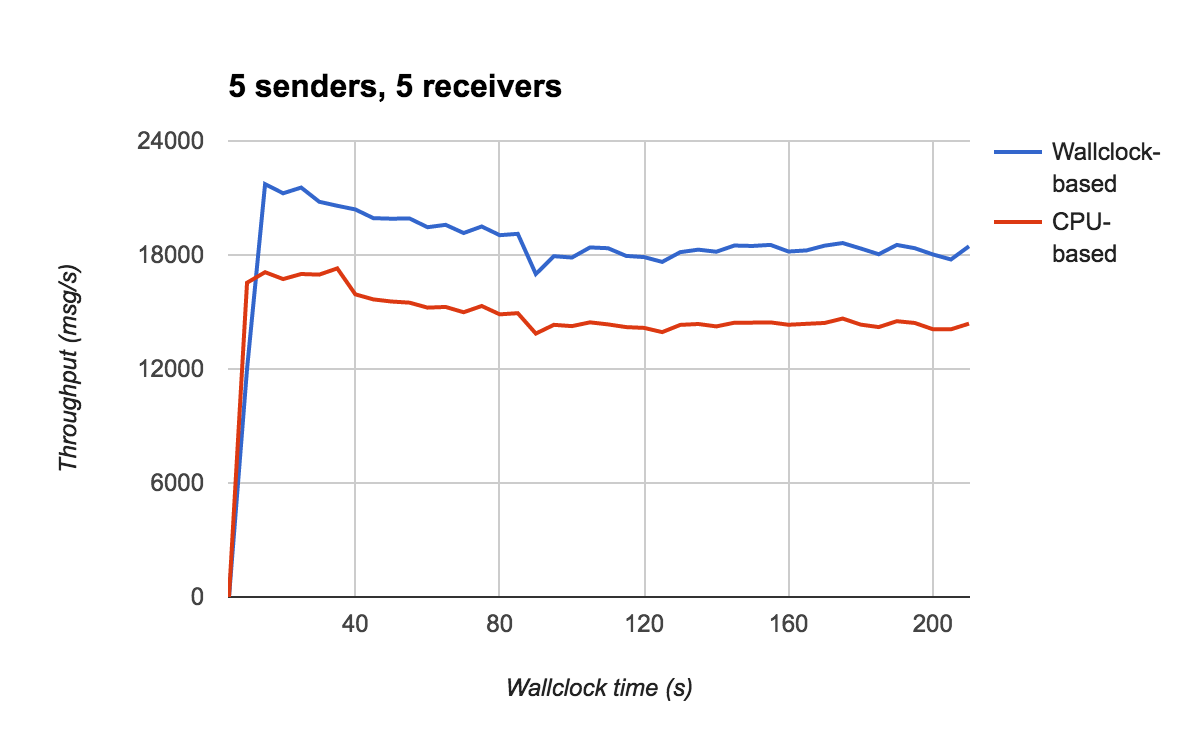
\includegraphics[width=\textwidth]{../transcripts/lipsum/5n5/5n5.png}
  \caption{5 send-receive pairs.}
  \label{fig:5n5}
\end{figure}

In Figure~\ref{fig:10n10}, at 10 client pairs, there is an odd dip at around $t=300s$.
\begin{figure}
  \centering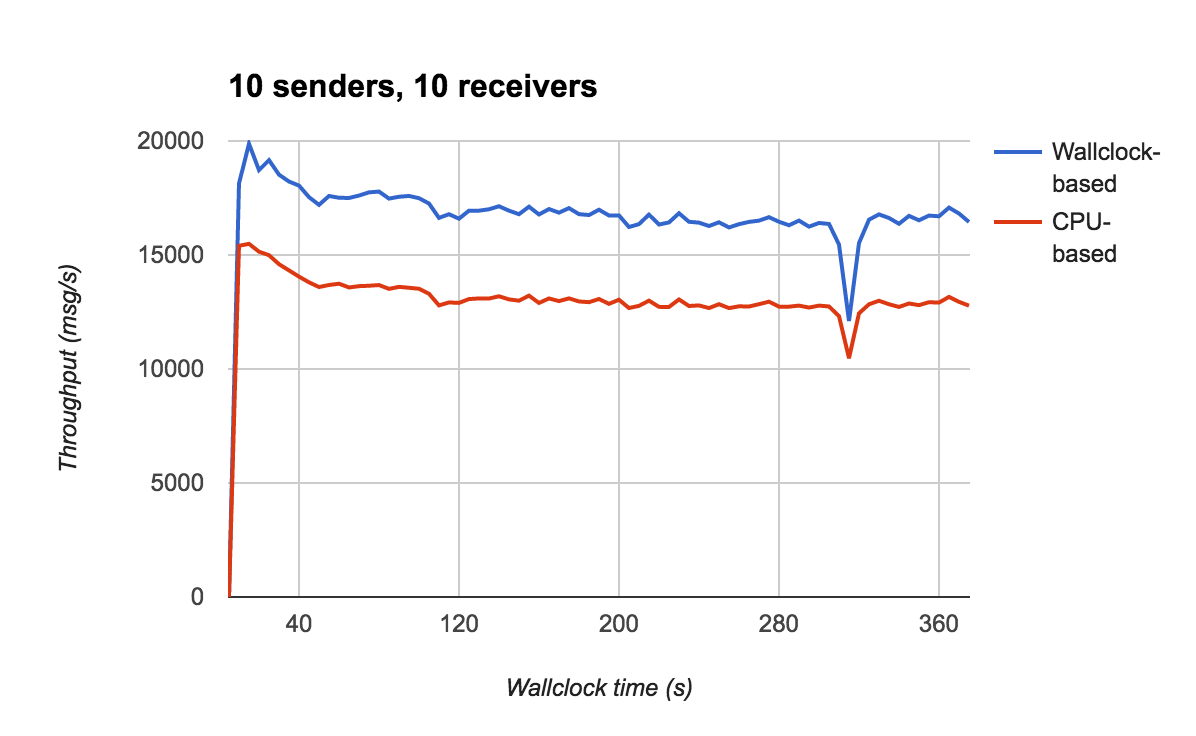
\includegraphics[width=\textwidth]{../transcripts/lipsum/10n10/10n10.png}
  \caption{10 send-receive pairs.}
  \label{fig:10n10}
\end{figure}

From 15 to 20 (Figure~\ref{fig:15n20}), we see much more chaotic behaviour from $t=300s$ that does not seem to stabilise:
\begin{figure}
  \centering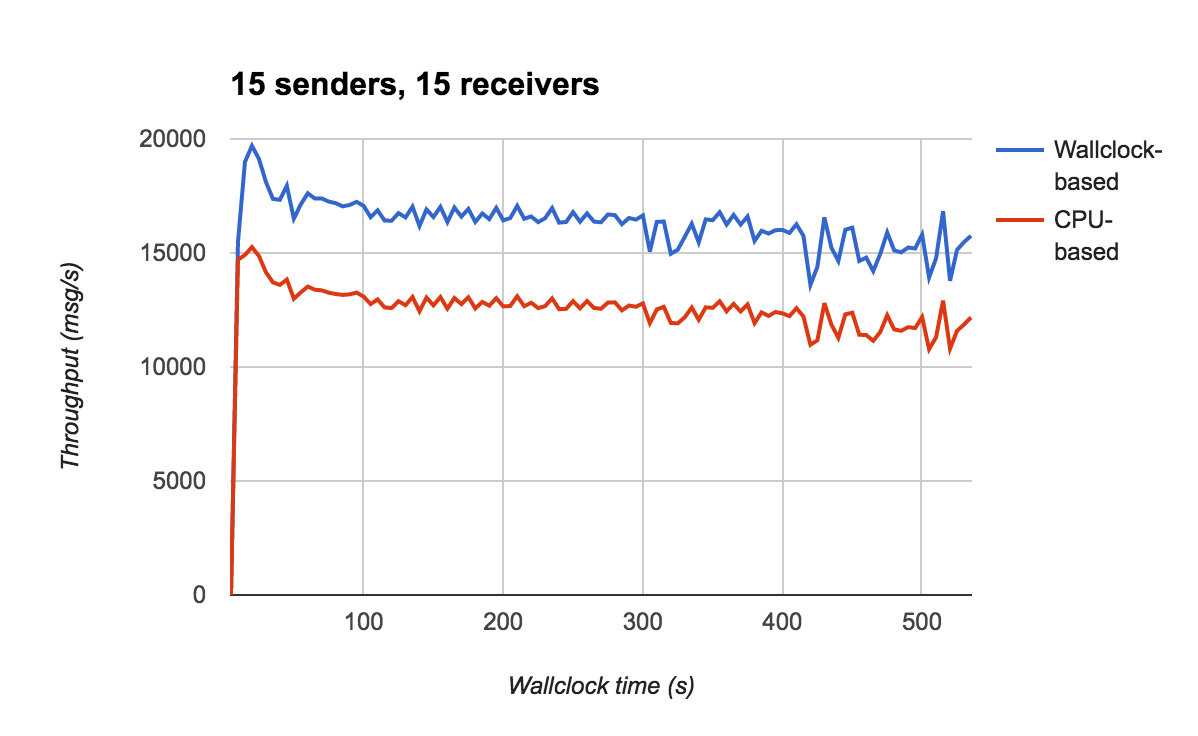
\includegraphics[width=\textwidth]{../transcripts/lipsum/15n15/15n15.png}

  \centering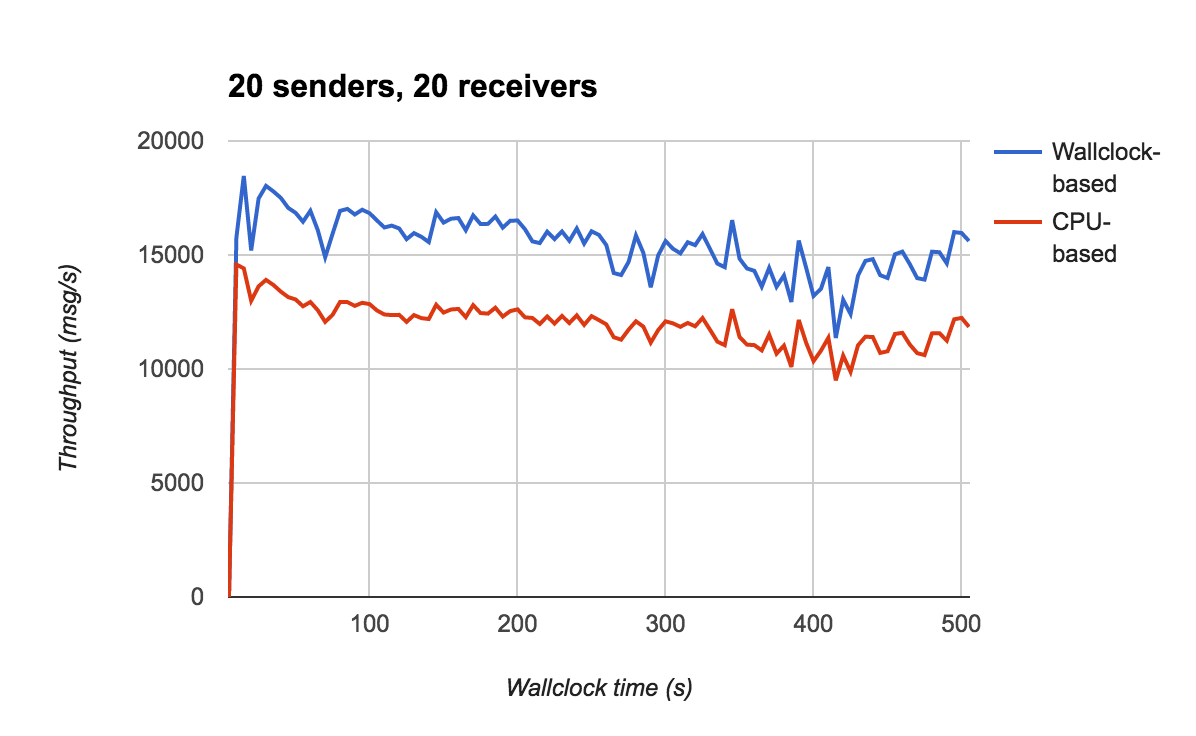
\includegraphics[width=\textwidth]{../transcripts/lipsum/20n20/20n20.png}
  \caption{20 send-receive pairs.}
  \label{fig:15n20}
\end{figure}

Stabilisation begins to return at 25 and beyond in Figure~\ref{fig:lots}. (Supposed to show 25-60)
\begin{figure}
  \centering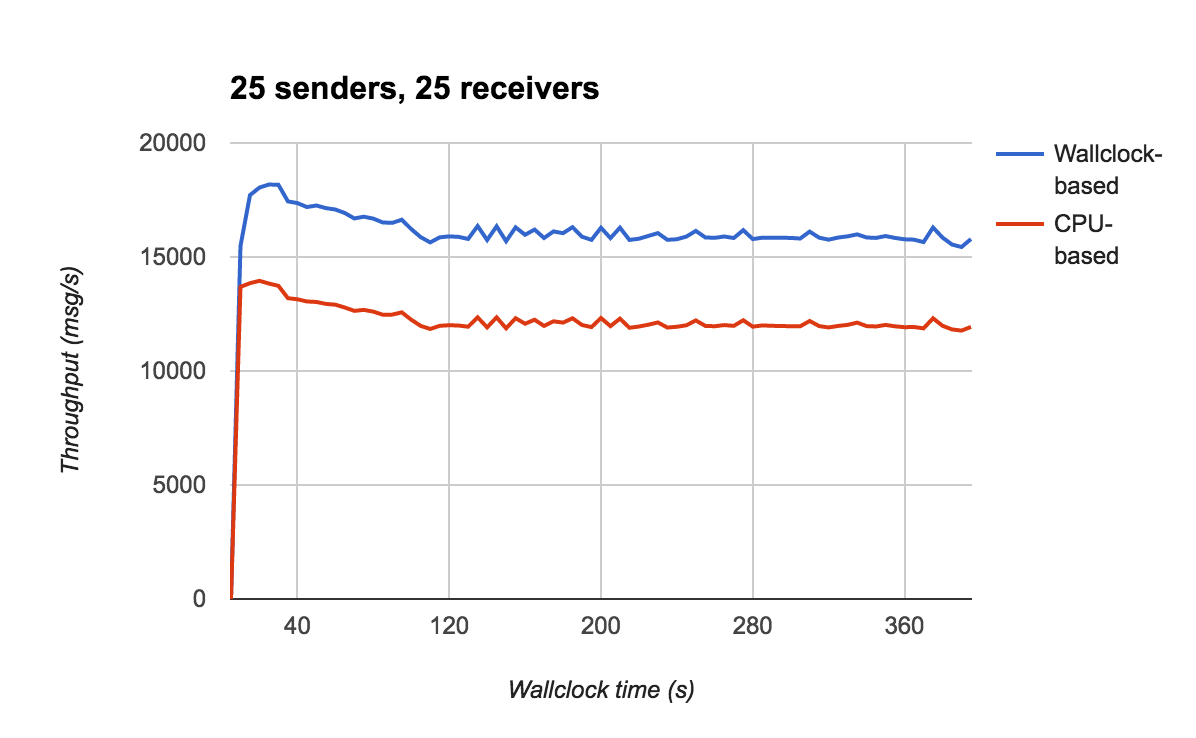
\includegraphics[width=\textwidth]{../transcripts/lipsum/25n25/25n25.png}

  \centering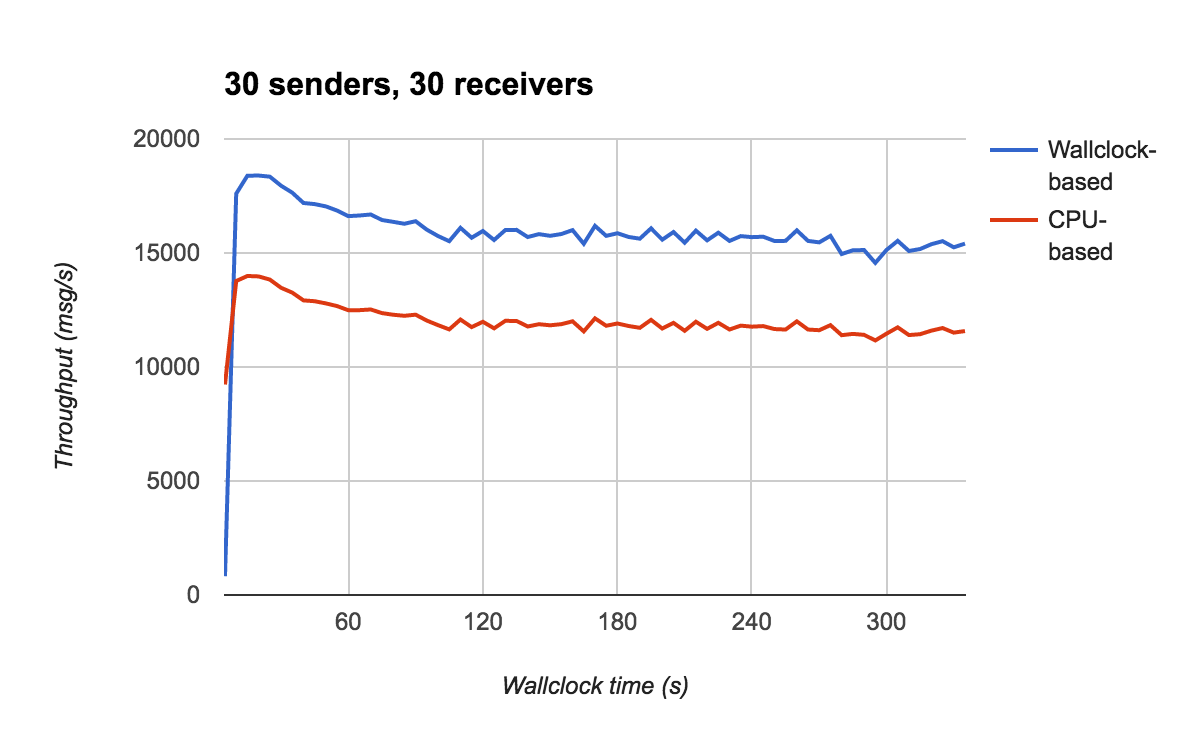
\includegraphics[width=\textwidth]{../transcripts/lipsum/30n30/30n30.png}
  \caption{30 send-receive pairs.}
  \label{fig:lots}
\end{figure}
\begin{figure}
  \centering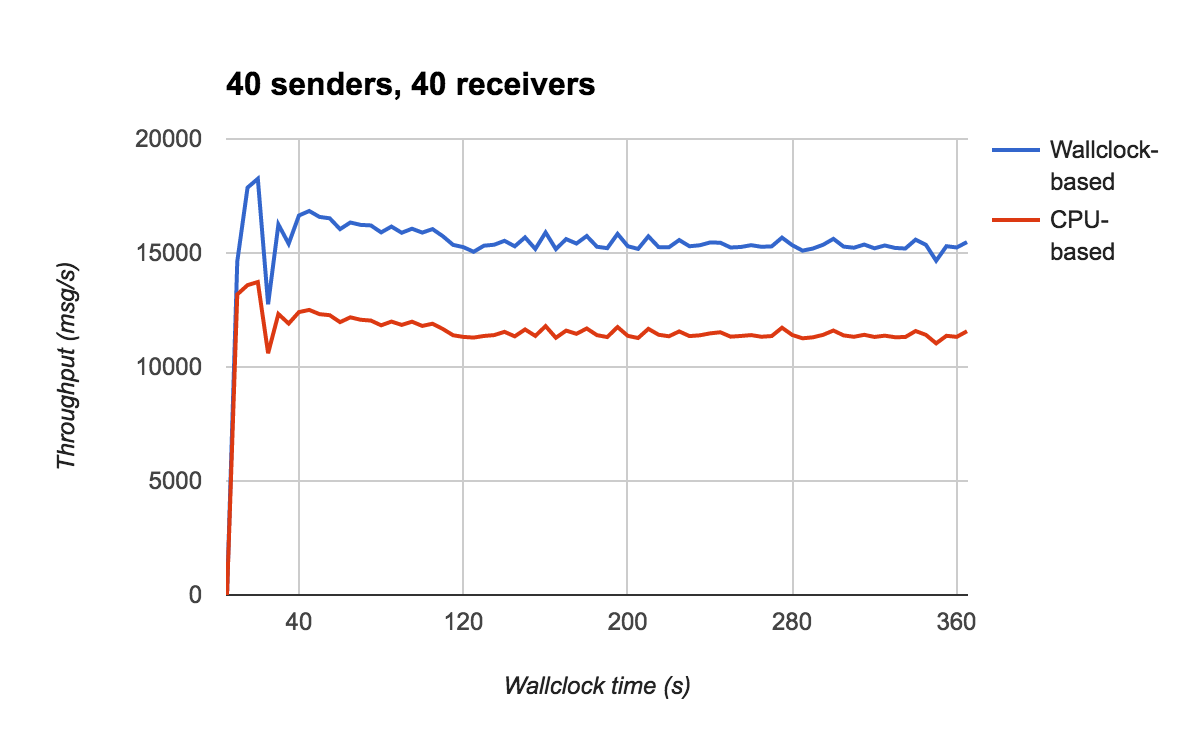
\includegraphics[width=\textwidth]{../transcripts/lipsum/40n40/40n40.png}

  \centering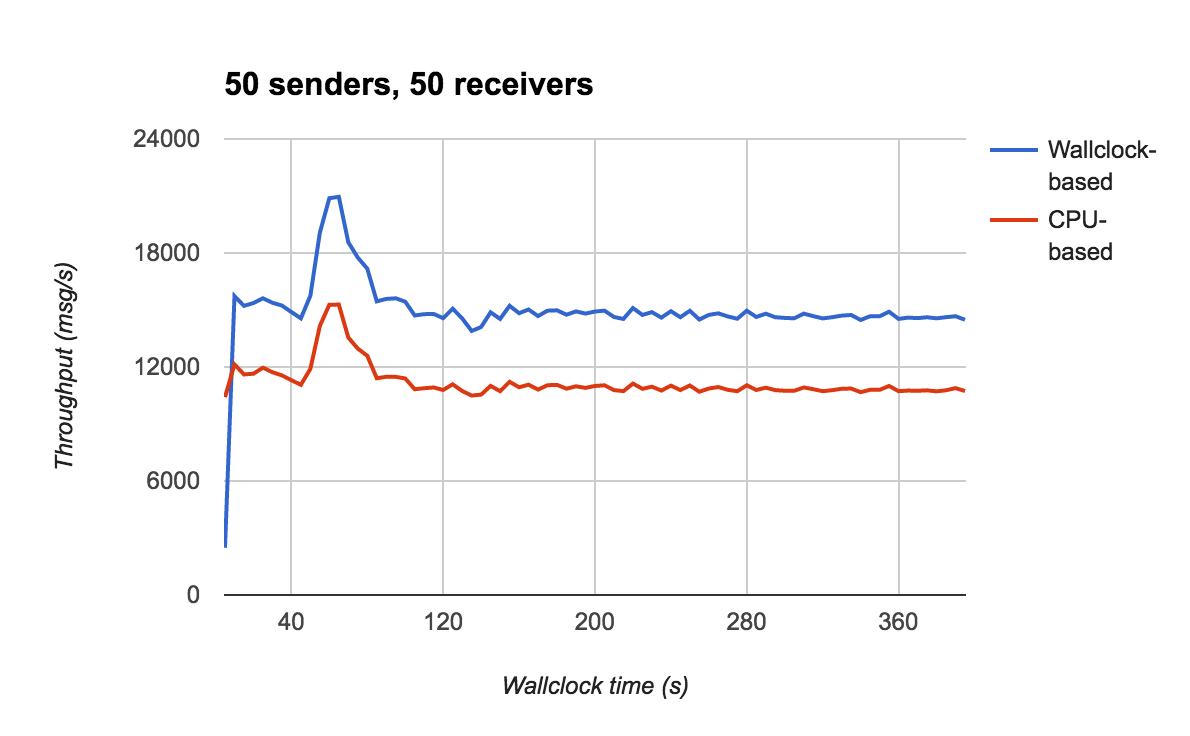
\includegraphics[width=\textwidth]{../transcripts/lipsum/50n50/50n50.png}
\end{figure}
\begin{figure}
  \centering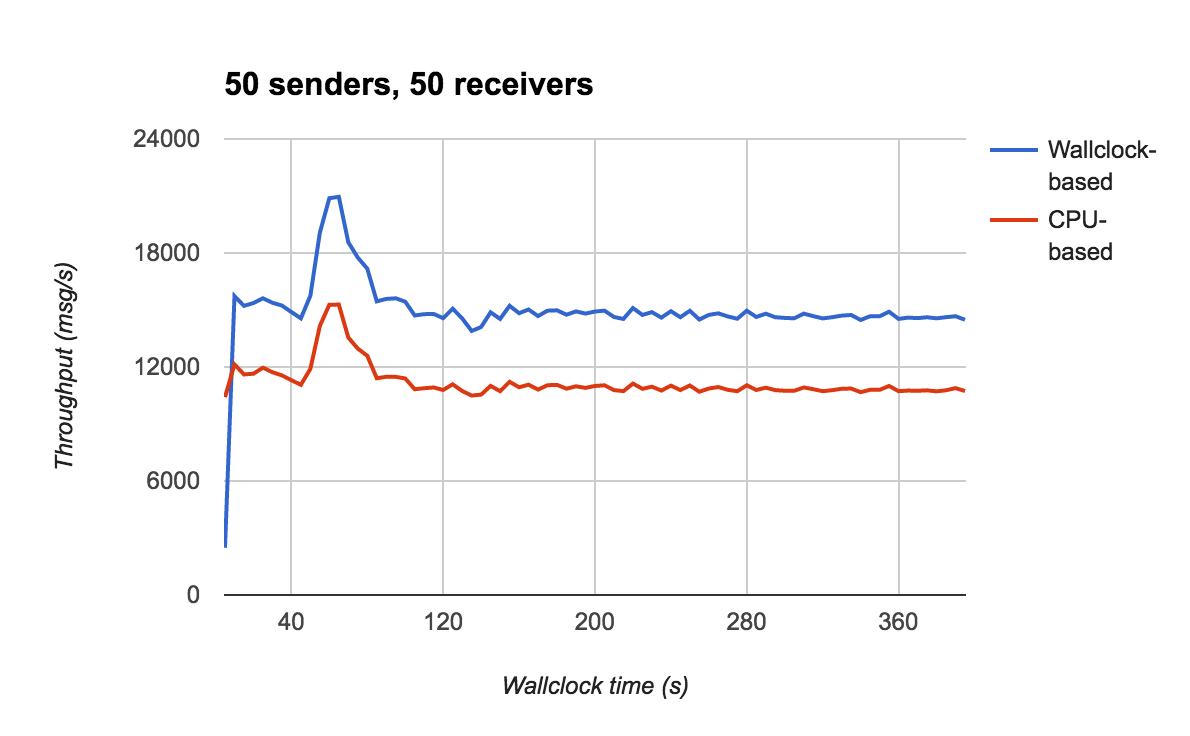
\includegraphics[width=\textwidth]{../transcripts/lipsum/50n50/50n50.png}

  \centering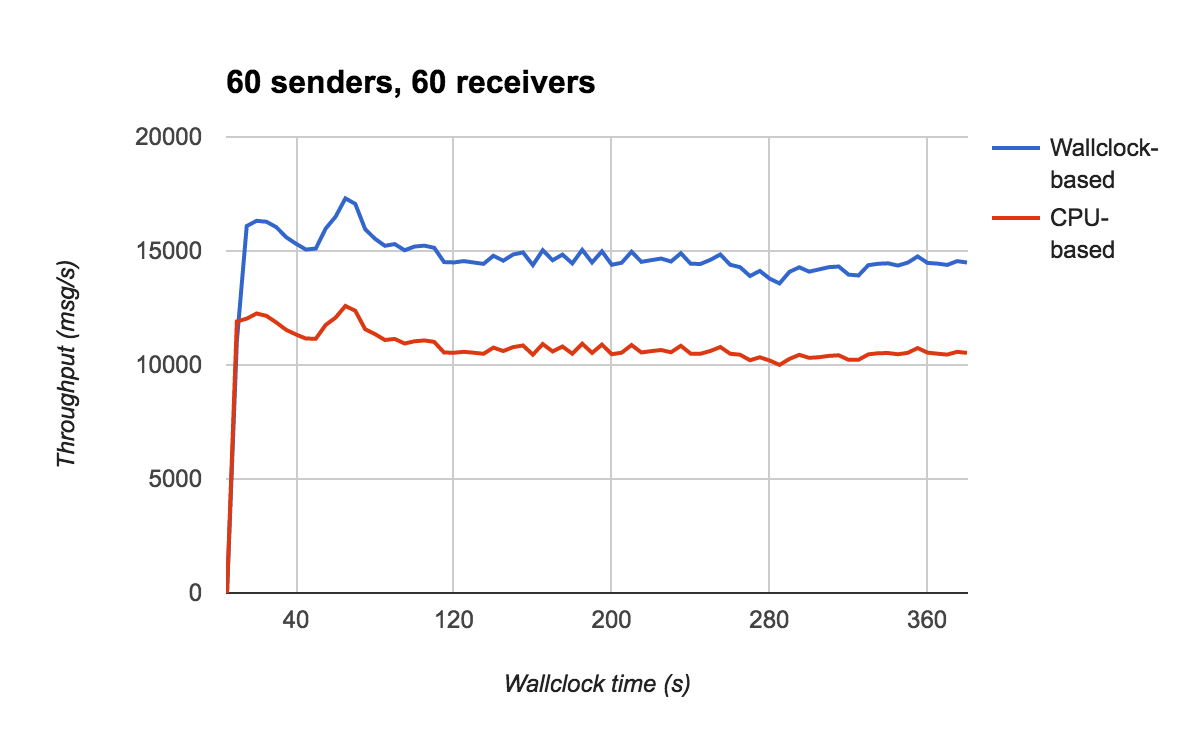
\includegraphics[width=\textwidth]{../transcripts/lipsum/60n60/60n60.png}
\end{figure}

I took the average of throughput samples in the stable-looking regions (or, for the chaotic graphs, the relatively stable-looking regions) and took the values as the ``operating throughputs'' of my server for these parameters. From this I obtained the indication of operating throughput as a function of client load shown in Figure~\ref{fig:summary}.

\begin{figure}
  \centering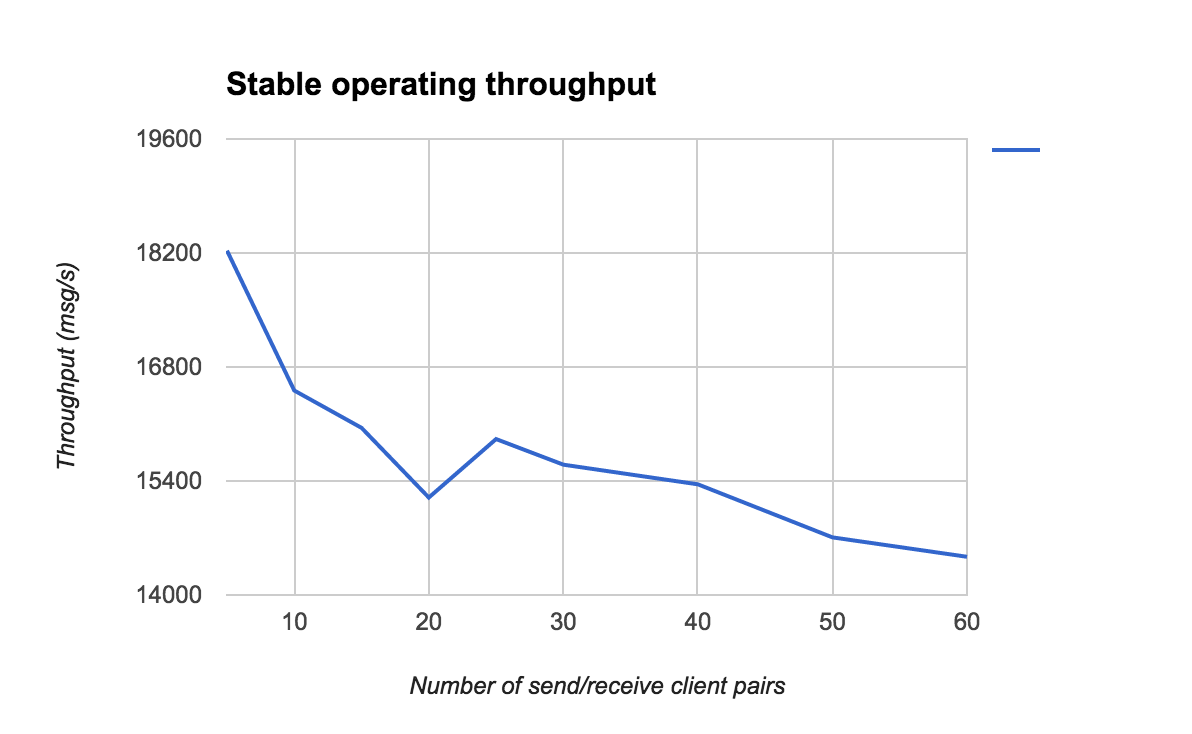
\includegraphics[width=\textwidth]{../transcripts/lipsum/throughp_clients.png}
  \caption{Effect of client load on operating throughput.}
  \label{fig:summary}
\end{figure}

\chapter{Conclusion}

\end{document}
